\documentclass{beamer} 
\usepackage{amsmath,amsthm}
\usepackage{graphicx,microtype,parskip}
\usepackage{caption,subcaption,multirow}
\usepackage{attrib}

\frenchspacing

\usetheme{default}
\usecolortheme{whale}

\setbeamertemplate{navigation symbols}{}

\setbeamercolor{title}{fg=blue,bg=white}

\setbeamercolor{block title}{fg=white,bg=gray}
\setbeamercolor{block body}{fg=black,bg=lightgray}

\setbeamercolor{block title alerted}{fg=white,bg=darkgray}
\setbeamercolor{block body alerted}{fg=black,bg=lightgray}


\title{The changing functional composition of the North American species pool}
\subtitle{ }
\author{Peter D Smits, Seth Finnegan}
\institute{Department of Integrative Biology, University of California -- Berkeley}
\date{}


\begin{document}


\begin{frame}
  \maketitle
\end{frame}


\begin{frame}
  \frametitle{Foundational assertion of conservation paleobiology }

  \begin{center}
    \begin{LARGE}
      By studying the \alert{past}, \\we can better predict the \alert{future}.
    \end{LARGE}
  \end{center}

\end{frame}


\begin{frame}
  \frametitle{What are we predicting?}
  
  \begin{center}
    \begin{LARGE}
      Extinction is \underline{hard} to predict, \\but is extremely important to conservation.
    \end{LARGE}
  \end{center}

\end{frame}


\begin{frame}
  \frametitle{Predicting extinction}

  \begin{itemize}[<+->]
    \item A taxon with a \alert{greater than average} global geographic range is likely to survive for longer than a taxon with \alert{less than average} global geographic range.
    \item A taxon's global geographic range can change over time.
    \item What happens to extinction risk as a taxon changes geographic range? How is extinction risk impacted if that taxon's global geographic range has recently \alert{increased} or \alert{decreased}?
  \end{itemize}

\end{frame}


\begin{frame}
  \frametitle{Encoding the past}

  \begin{itemize}
    \item Change in geographic range between current observation and previous observation.
    \item Average global temperature at time of previous observation (Mg/Ca isotope).
    \item Age in millions of years at time of observation.
  \end{itemize}

\end{frame}


\begin{frame}
  \frametitle{Data being analyzed}

  \begin{columns}
    \begin{column}{0.5\textwidth}
      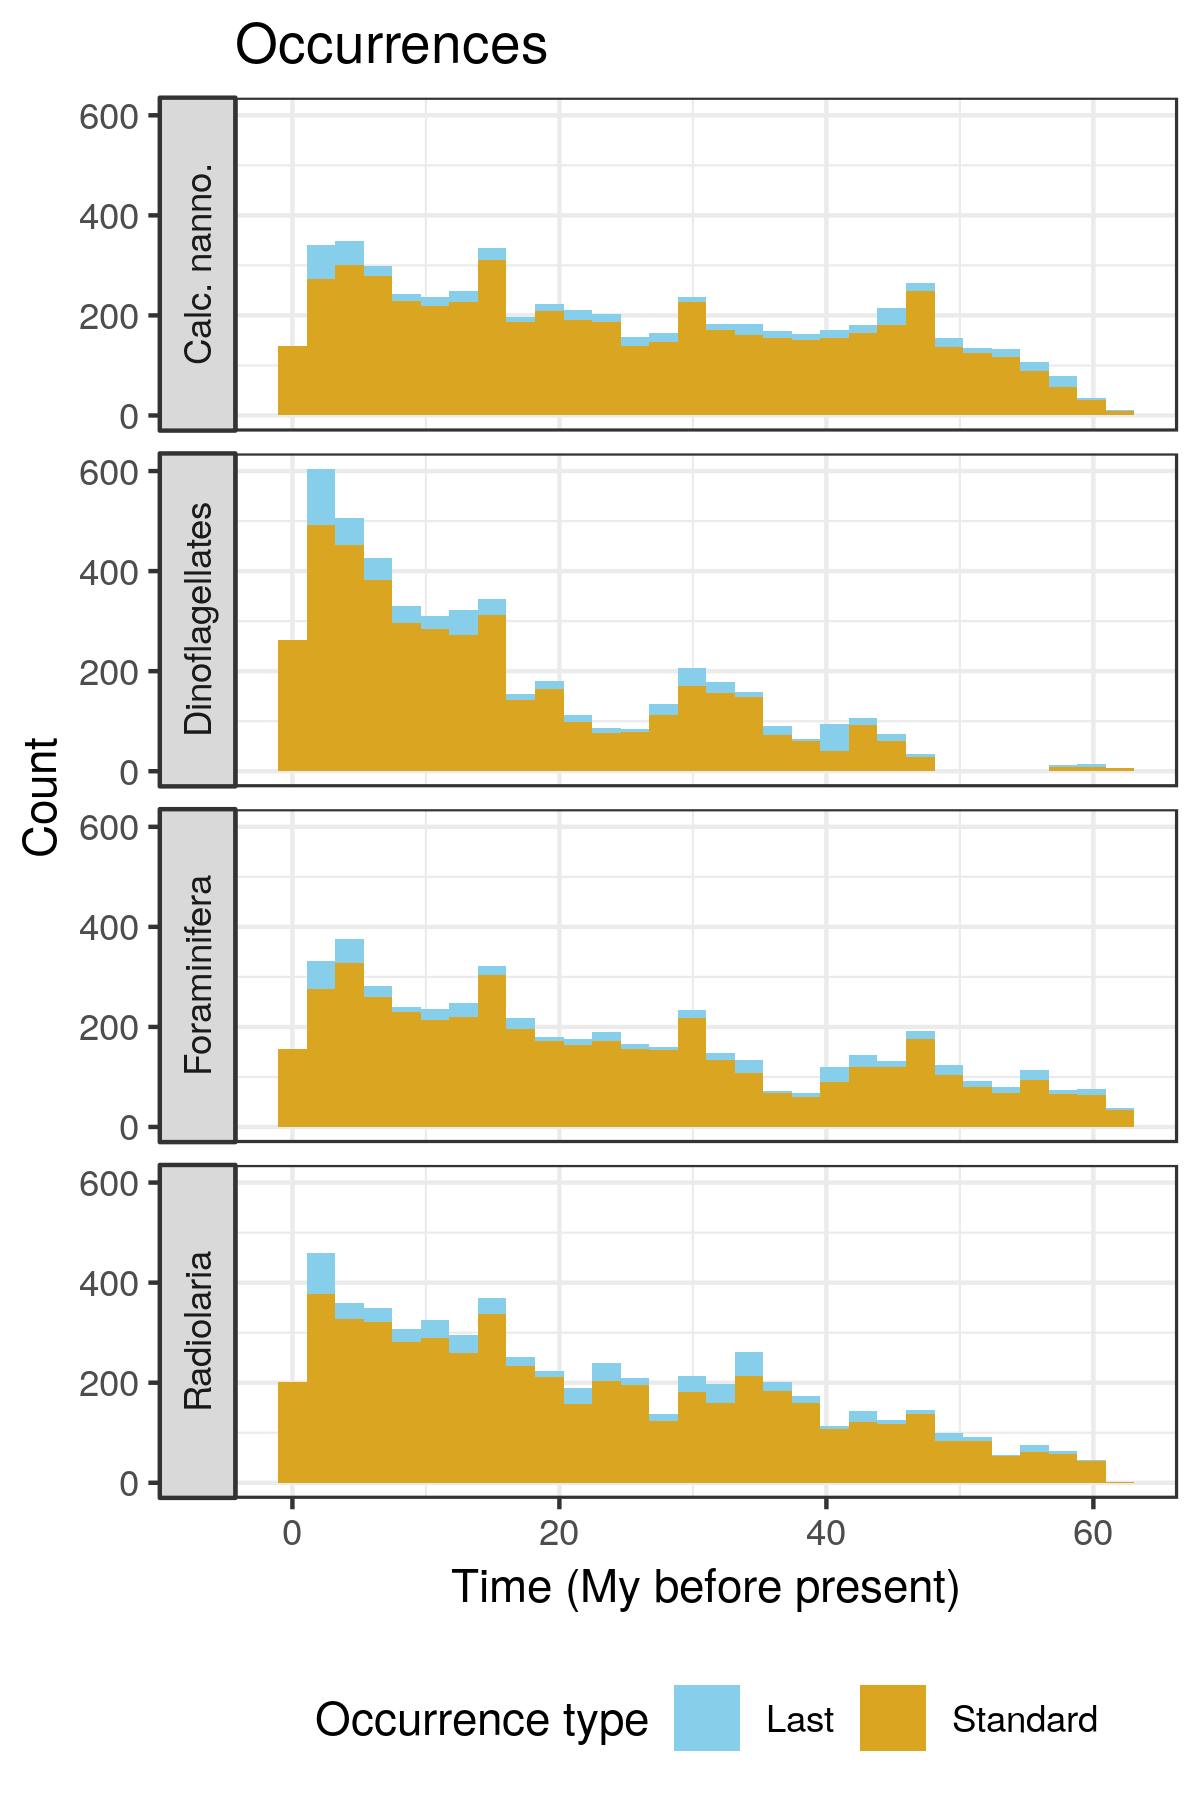
\includegraphics[width=\textwidth,height=\textheight,keepaspectratio=true]{../results/figure/occ_time_label}
    \end{column}
    \begin{column}{0.5\textwidth}
      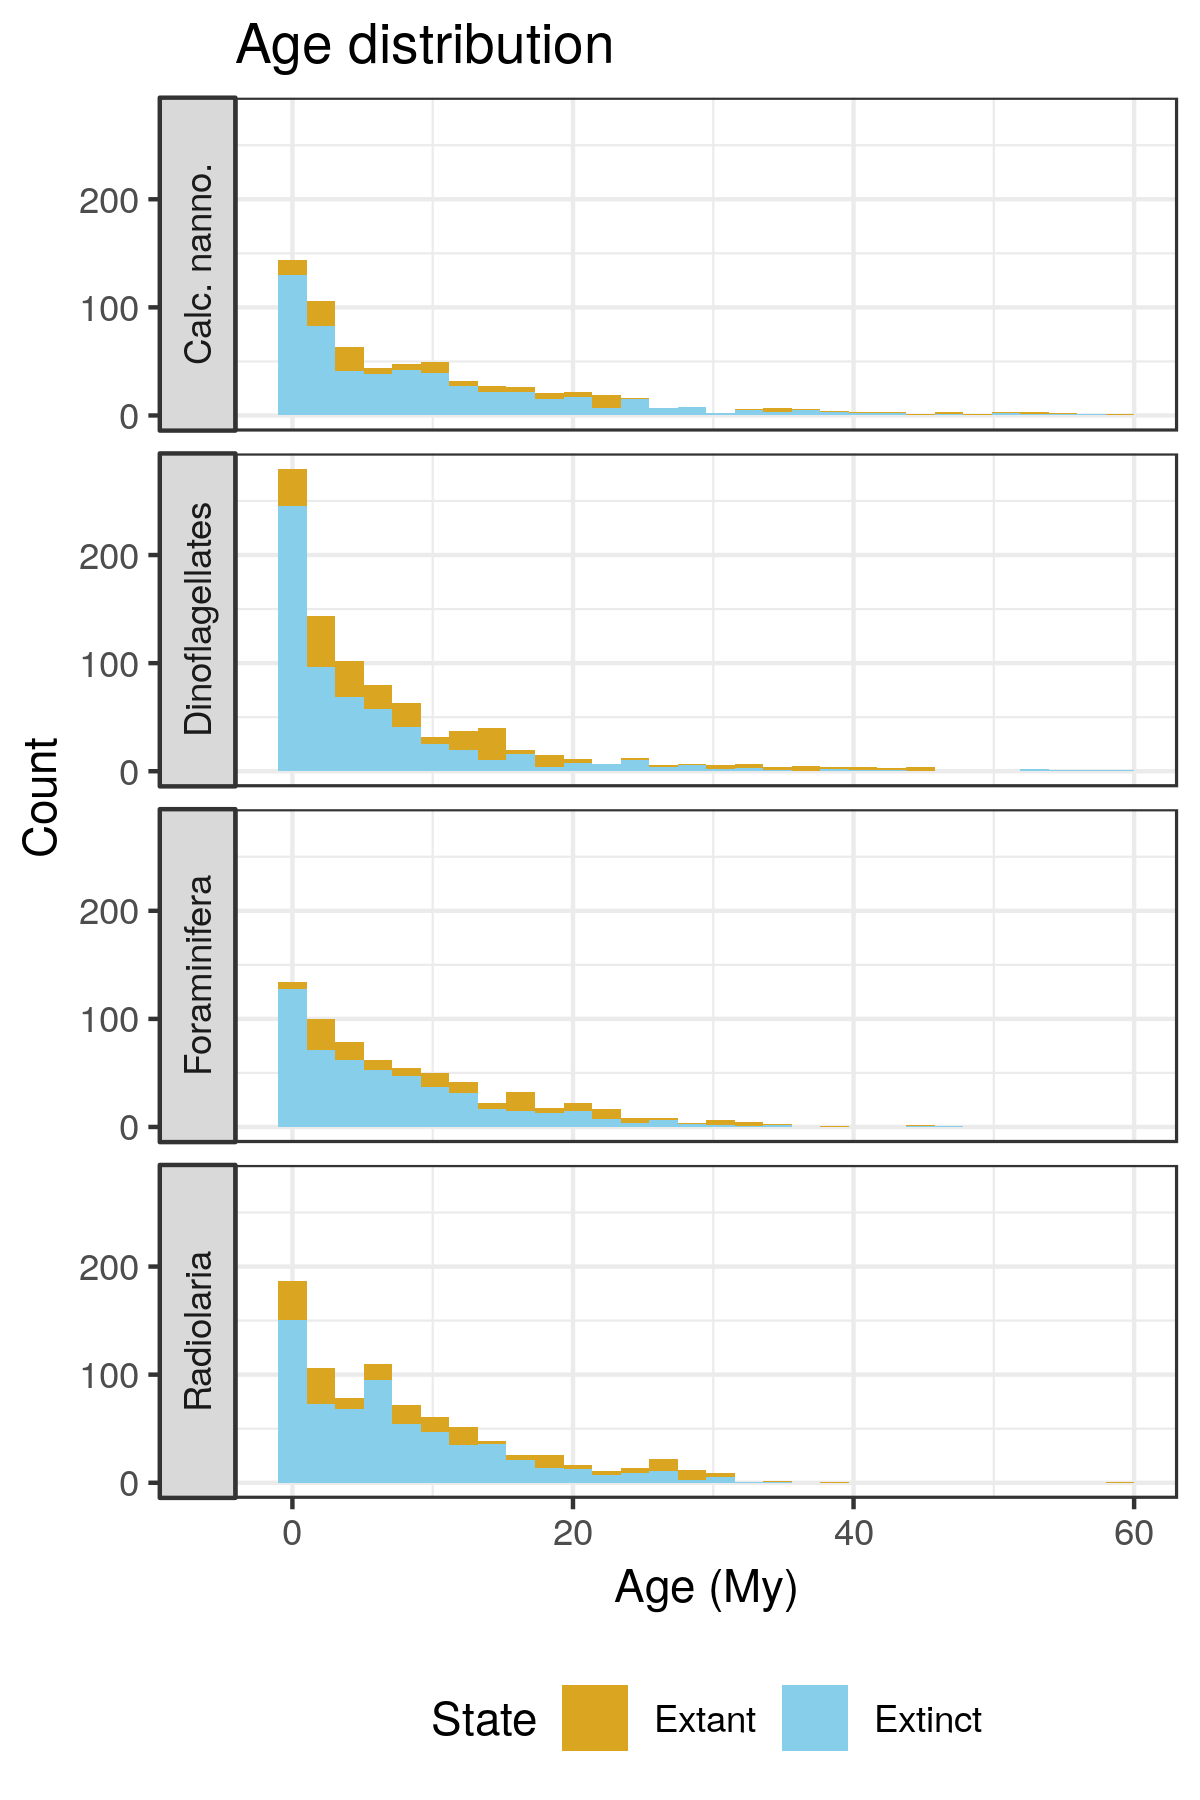
\includegraphics[width=\textwidth,height=\textheight,keepaspectratio=true]{../results/figure/age_label}
    \end{column}
  \end{columns}

\end{frame}


\begin{frame}
  \frametitle{How we're analyzing the data}

  \begin{itemize}[<+->]
    \item Predictors: geographic range, change in geographic range, global temperature, lag of global temperature.
    \item Bayesian discrete-time survival model.
      \begin{itemize}
        \item<.-> Bernoulli response distribution.
        \item<.-> Time/phylum varying intercepts and slopes.
        \item<.-> Taxon age as non-nested varying intercept.
      \end{itemize}
    \item \alert{Compare} models using WAIC/LOOIC.
    \item Explore model \alert{adequacy} using posterior predictive distribution.
    \item Estimate \alert{predictive performance} using \(k\)-fold cross-validation.
  \end{itemize}

\end{frame}


\begin{frame}
  \frametitle{A conceptual model for predicting extinction}

\end{frame}


\begin{frame}
  \frametitle{A statistical model for predicting extinction}

\end{frame}


\begin{frame}
  \frametitle{Comparing our models}

  % table of waic/looic values
  %   se values come out second to demonstrate how all virtually identical

\end{frame}


\begin{frame}
  \frametitle{Cross-validation results}

  % figure comparing in-sample AUC to out-of-sample AUC
  %   they are similar

\end{frame}


\begin{frame}
  \frametitle{Tracking extinction risk over time}
  
\end{frame}


\begin{frame}
  \frametitle{Overall covariate effects}  

\end{frame}


\begin{frame}
  \frametitle{Covariate effects over time}  

\end{frame}


\begin{frame}
  \frametitle{Effects of age on extinction risk}

\end{frame}


\begin{frame}
  \frametitle{Summary}

\end{frame}


\begin{frame}
  \frametitle{Conclusions}

\end{frame}


\begin{frame}
  \frametitle{Acknowledgements}

\end{frame}


\end{document}
